% !TeX root = ex2.tex
\subsection{Video and Images}

\subsubsection{Video to images}

\paragraph{Problem} Given a video, convert it into constituent images

\paragraph{Experiments \& Learning} Experiments performed are listed below

\begin{enumerate}
    \item Giving user input to the program: Tried using the \texttt{input} \href{https://docs.python.org/3/library/functions.html#input}{built-in} to read from console. Finally settled at using \href{https://docs.python.org/3.10/library/argparse.html#module-argparse}{argparse}. Learned how to parse parameters professionally using argparse.
    \item Using \href{https://docs.opencv.org/4.x/d8/dfe/classcv_1_1VideoCapture.html}{VideoCapture} and \href{https://docs.opencv.org/4.x/d8/dfe/classcv_1_1VideoCapture.html#a473055e77dd7faa4d26d686226b292c1}{read} functions to fetch images from a video file, and writing images to disk using \href{https://docs.opencv.org/4.x/d4/da8/group__imgcodecs.html#gabbc7ef1aa2edfaa87772f1202d67e0ce}{imwrite}. Some experiments were run where the output prefix directory did not exist, so added the code to create the directory first.
\end{enumerate}

\paragraph{Solution}

Download video from \href{https://github.com/opencv/opencv/blob/master/samples/data/vtest.avi}{here} and store as \texttt{./videos/vtest.avi}. Then run the following

\begin{verbatim}
    python .\vid_to_imgs.py -n 10
\end{verbatim}

The code is shown in listing \ref{lst:q2-vid-to-imgs}. Output is in figure \ref{fig:q2-v2i-seq}.

\lstinputlisting[language=python, caption={vid\_to\_imgs.py}, label=lst:q2-vid-to-imgs]{../python/vid_to_imgs.py}

The above script (listing \ref{lst:q2-vid-to-imgs}) gives the following output (along with a GUI window to show the images of the video)

\begin{verbatim}
    Folder ./out is being created
    Reached 10 frames
    Wrote 10 frames under ./out/img*.jpg
\end{verbatim}

\begin{figure}[t]
    \centering
    \begin{subfigure}[b]{0.3\textwidth}
        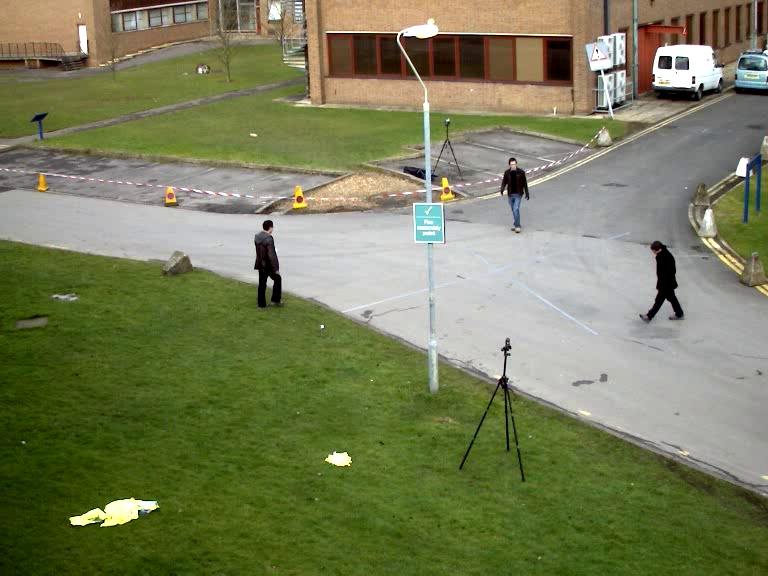
\includegraphics[width=\textwidth]{../out/img1.jpg}
        \caption{Image 1}
    \end{subfigure}
    \begin{subfigure}[b]{0.3\textwidth}
        \includegraphics[width=\textwidth]{../out/img5.jpg}
        \caption{Image 5}
    \end{subfigure}
    \begin{subfigure}[b]{0.3\textwidth}
        \includegraphics[width=\textwidth]{../out/img10.jpg}
        \caption{Image 10}
    \end{subfigure}
    \caption{Sequence of images}
    \label{fig:q2-v2i-seq}
    \small
        First, fifth, and tenth image in the 10-image sequence produced by listing \ref{lst:q2-vid-to-imgs}.
\end{figure}

\subsubsection{Images to Video}

\paragraph{Problem}
Given a folder with images, create a video where the FPS (frame rate) can be adjusted

\paragraph{Experiments \& Learning}
Experiments performed are listed below

\begin{enumerate}
    \item Getting images into the program: It was decided that the user will place the images, labelled in a sorted order (numerically), in a dedicated folder. For this demo, the folder name is \texttt{./seq}
    \item All user inputs are given through \texttt{argparse}
    \item FPS will be handled by the \texttt{VideoWriter} in the saved video file. However, the preview FPS has to be manually adjusted (using \texttt{waitKey} delay)
\end{enumerate}

\paragraph{Solution}
Store images in a numerical order from $1$.jpg to $\textup{N}$.jpg (where $\textup{N}$ is any number) in a dedicated folder, like \texttt{./seq}. Then run the following (for 5 FPS)

\begin{verbatim}
    python .\imgs_to_vid.py -i "./seq" -f 5.0 -o "./out-5.avi"
\end{verbatim}

The code is shown in listing \ref{lst:q2-imgs-to-vid}. A snapshot of the generated video is shown in figure \ref{fig:sfig-q2-i2v-5fps}.
The following is an example for 10 FPS

\begin{verbatim}
    python .\imgs_to_vid.py -i "./seq" -f 10.0 -o "./out-10.avi"
\end{verbatim}

A snapshot of the video generated is shown in figure \ref{fig:sfig-q2-i2v-10fps}. See figure \ref{fig:q2-i2v-imgs} for more information.

\lstinputlisting[language=python, caption={imgs\_to\_vid.py}, label=lst:q2-imgs-to-vid]{../python/imgs_to_vid.py}

\begin{figure}[t]
    \centering
    \begin{subfigure}[b]{0.45\textwidth}
        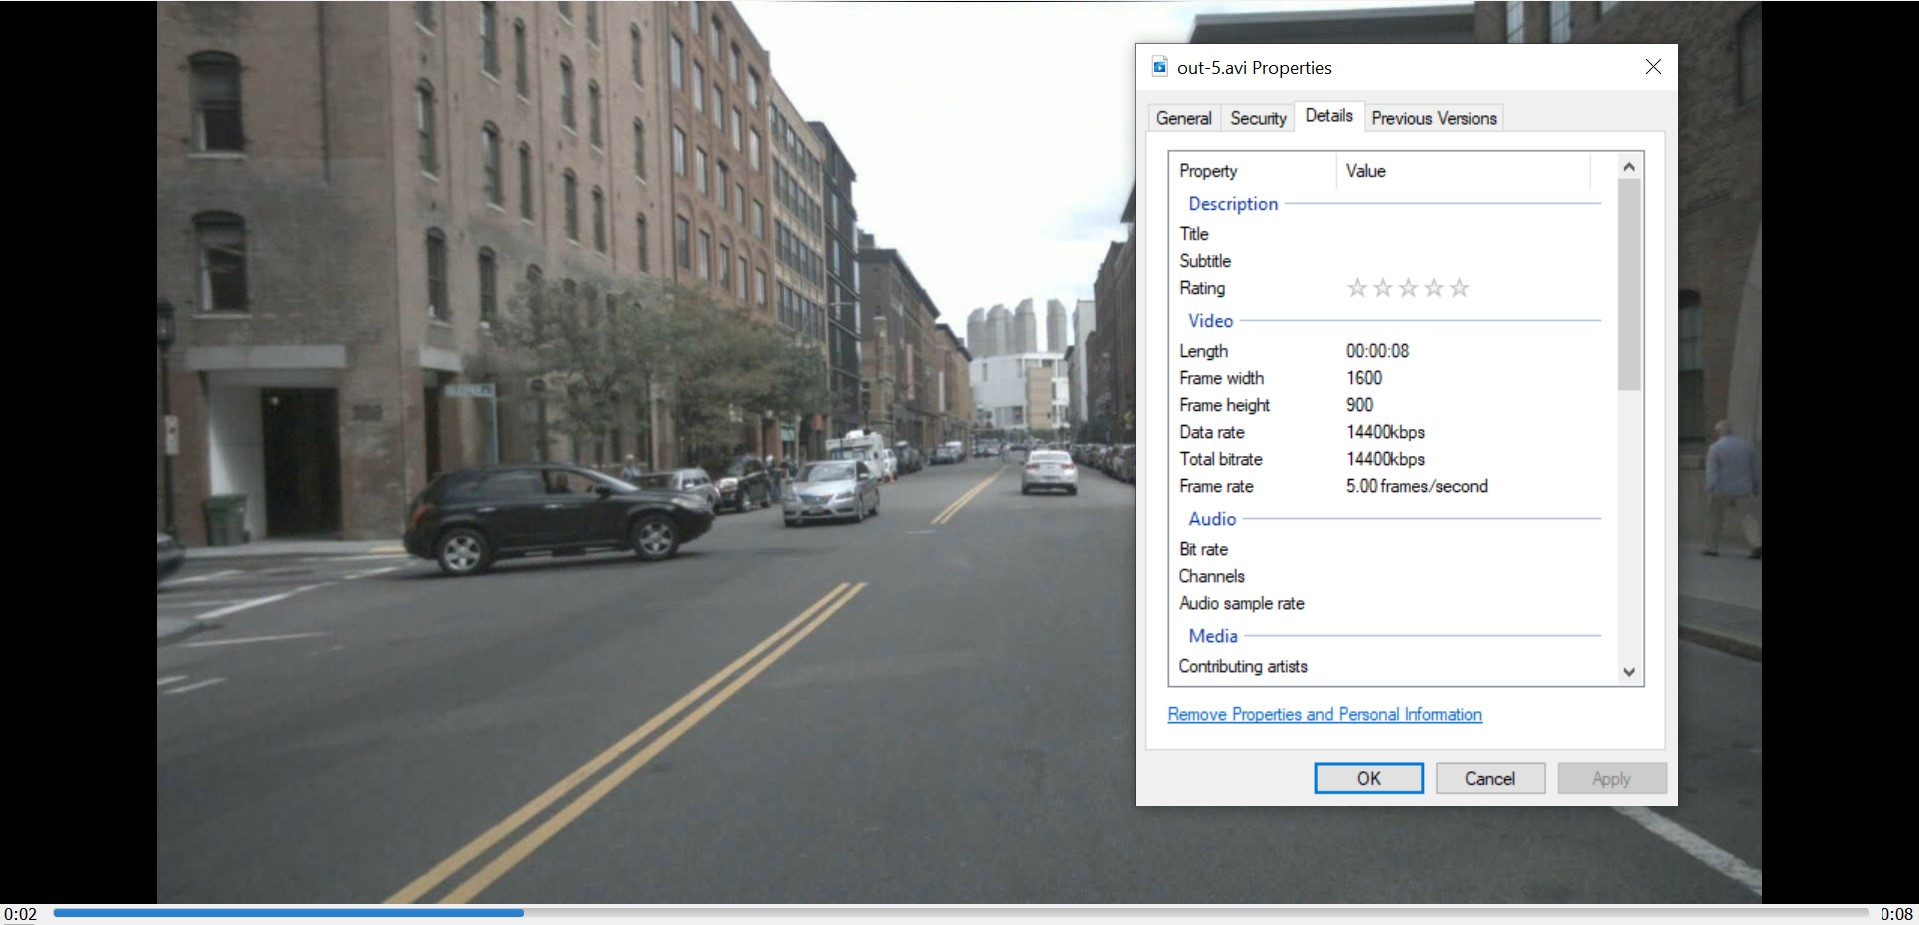
\includegraphics[width=\textwidth]{q2-im2vid-5fps.jpg}
        \caption{5 FPS}
        \label{fig:sfig-q2-i2v-5fps}
    \end{subfigure}
    \begin{subfigure}[b]{0.45\textwidth}
        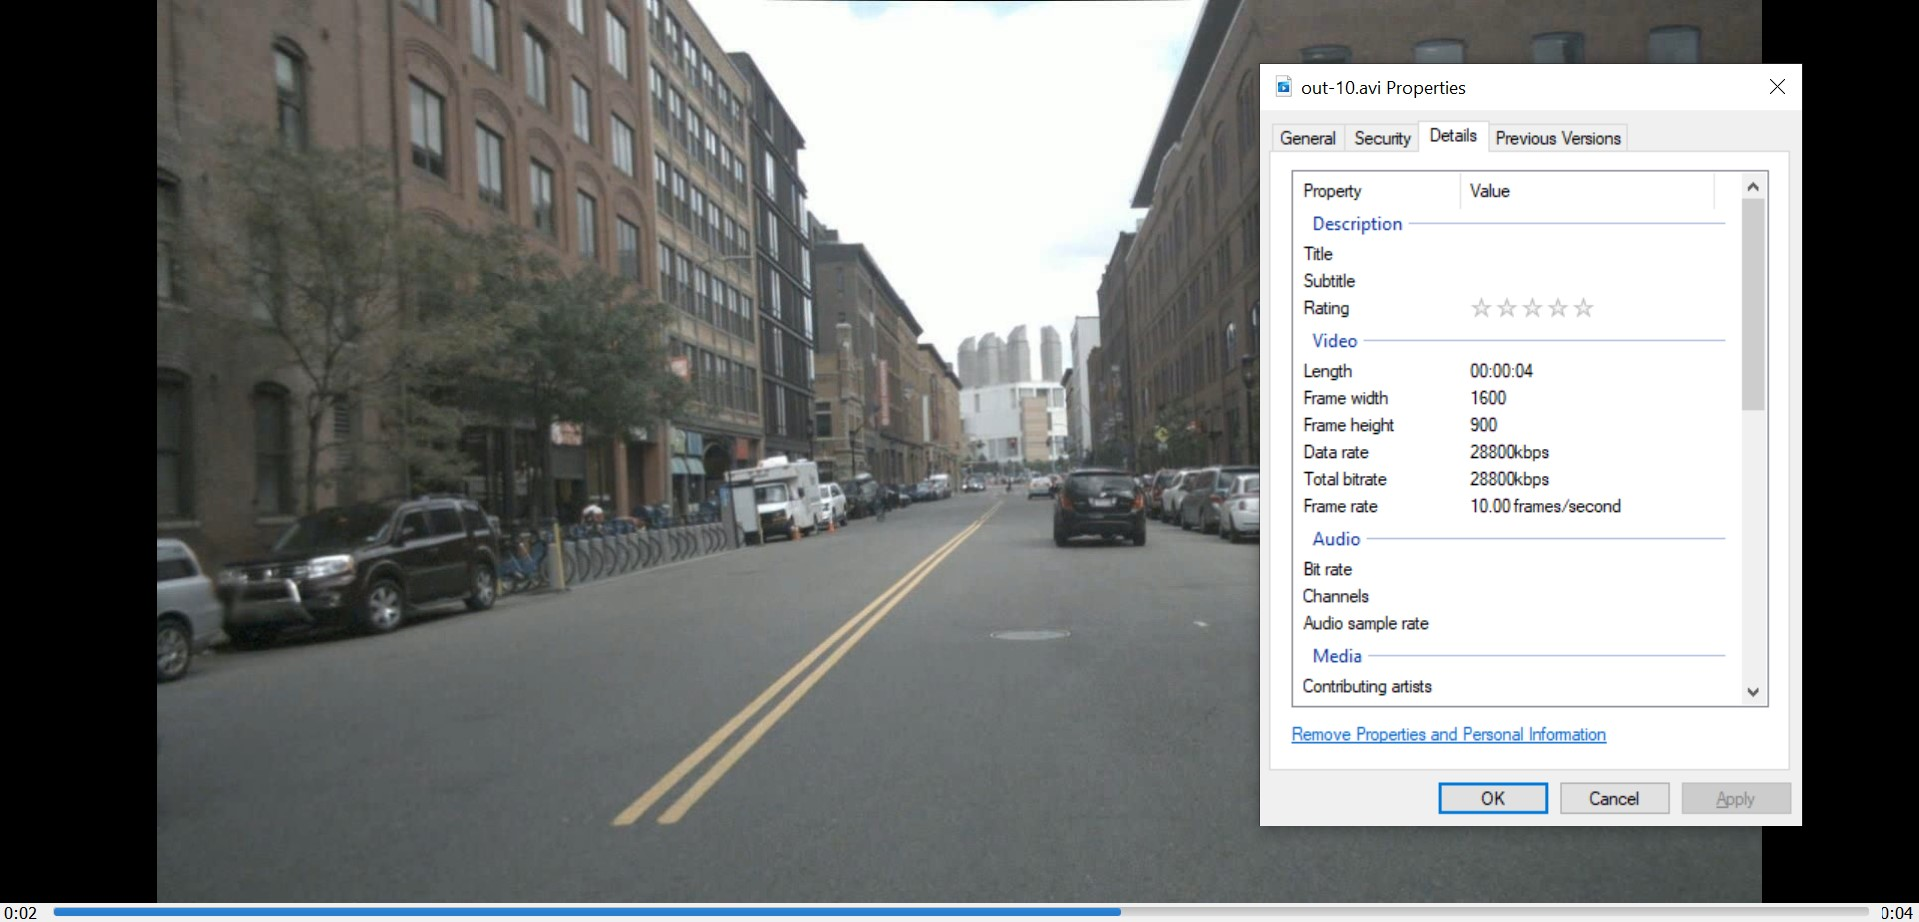
\includegraphics[width=\textwidth]{q2-im2vid-10fps.jpg}
        \caption{10 FPS}
        \label{fig:sfig-q2-i2v-10fps}
    \end{subfigure}
    \caption{Saved videos}
    \label{fig:q2-i2v-imgs}
    \small
        Image \ref{sub@fig:sfig-q2-i2v-5fps} is a screenshot of the \texttt{5 FPS} playback (see the properties and the video frame). Image \ref{sub@fig:sfig-q2-i2v-10fps} is a screenshot of the \texttt{10 FPS} playback. Notice that the \texttt{10 FPS} version is faster, therefore a greater number of frames elapsed (for the 2 second point) compared to the \texttt{5 FPS} version.
\end{figure}
